\section{Introduction}
\label{section_search_intro}
In the previous chapters we have laid the groundwork for the main event: searching for new asteroids in the ZTF dataset.
Here is an outline of the search process, which will be elaborated in greater detail in the sections below.
The search is initialized with a set of candidate orbital elements that is generated randomly based on the orbital elements of known asteroids.
The orbits are integrated over the unique times present in the ZTF data, 
and the subset of ZTF detections within a threshold (2 degrees) of each candidate element is assembled.

A custom Keras model class called \tty{AsteroidSearch} performs a search using gradient descent.
This search optimizes an objective function that is closely related to the joint log likelihood of the orbital elements
as well a set of parameters describing a mixture model.
The mixture model describes the probability distribution of the squared distance over the threshold as a mixture of hits and misses.
Hits are modeled as following an exponential distribution, and misses are modeled as being distributed uniformly.
A set schedule of adaptive training is run.  
This training schedule has alternating periods of training just the mixture parameters at a high learning rate
and jointly training the mixture parameters and orbital elements.

At the conclusion of the training process, we tabulate ``hits'' which are here defined as ZTF detections that are within 10 arc seconds of the predicted direction.
All the fitted orbital elements are saved along with summary statistics of how well they were fit including the mixture parameters.
The most important indicator is the number of hits.
Candidate orbital elements with at least 5 hits are deemed noteworthy and candidates with 8 or more hits are deemed to have been provisionally fit.
The search program also saves the ZTF detections associated with each fitted orbital element.

I demonstrate the effectiveness of this method in a series of increasingly difficult tests.  
The easier tests involve recovering the orbital elements of known asteroids that have many hits in the ZTF dataset.
The most difficult task is to identify the orbital elements of new asteroids by searching the subset of ZTF detections that don't match the known asteroid catalogue.
In particular, the five tasks presented are
\begin{itemize}
\item recover the elements of known asteroids starting with the exact elements, but uninformed mixture parameters
\item recover the elements of known asteroids starting with lightly perturbed elements
\item recover the elements of known asteroids starting with heavily perturbed elements
\item ``rediscover'' the elements of known asteroids starting with randomly initialized elements
\item discover the elements of unkown asteroids starting with randomly initialized elements
\end{itemize}
The search process presented passes the first three test with varying degrees of success, recovering 64, 37 and 11 elements respectively out of the 64 candidates.
The search for known asteroids from random initializations has 1 success on the first batch of 64 and is eventually run on a large scale.
The search for previously unknown asteroids yields \todo{N} orbital elements that I claim belong to real but uncatalogued asteroids.

I tested the quality of the results by comparing the fitted orbital elements to the known orbital elements on two metrics.
The most important indicator is to compare the orbits on a set of representative dates and compute the mean squared difference in the position in AU.
A secondary metric is to compare the orbital elements.  
This is done with a metric that standardizes each element and assigns it an importance score.
Both of these metrics show excellent agreement of the recovered orbital elements with the existing elements in the asteroid catalogue.

\section{Generating Candidate Orbital Elements}
\label{section_candidate_elements}
The search is initialized with a batch of candidate orbital elements. 
The batch size is a programming detail; I selected $n=64$.
The choice of initial orbital elements is critically important to the search.
Unlike with other problems, where in theory there is often one globally correct answer 
that might or might not be reachable depending on the initialization, 
the number of local maxima in the objective function here will be at least the number of real asteroids adequately represented in the data.
Based on the last chapter, that means there are over 100,000 local maxima in the objective function.

In this work I use a simple strategy of random initializations.
Improving on this initiailization strategy is the most important item of future work.
I had originally planned to upgrade this to a more intelligent initialization but unfortunately ran out of time.
Random initialization would be nearly hopeless if we had no information about the probability distribution of orbital elements.
But because we have access to large asteroid catalogue, it is feasible to generate plausible candidate elements.

The random initialization strategy breaks the six orbital elements into two categories: empirical and uniform.
The elements $a$, $e$, $i$ and $\Omega$ are sampled from the empirical distribution.
To be more precise, four random indices $j_{a}$, $j_{e}$, $j_{i}$ and $j_{\Omega}$ between 1 and 733,489 are selected, 
and the initialization is done by setting e.g. $a_{j}$ equal to the semi-major axis of the known asteroid with number $j_{a}$.
The two orbital elements $M$ and $\omega$ are initialized uniformly at random on the interval $[0, 2\pi)$.
We know from Kepler's second law (equal time in equal area) that the mean anomaly $M$ is linear in time,
so we have a solid theoretical argument for sampling it uniformly.
Once $M$ is determined, it is converted to $f$ using \tty{REBOUND}.
I will show empirically that the argument of perhelion $\omega$ appears to be distributed very close to uniformly as well.

Here are charts for selected mathematical transformations of orbital elements.
\begin{figure}[hbt!]
\begin{center}
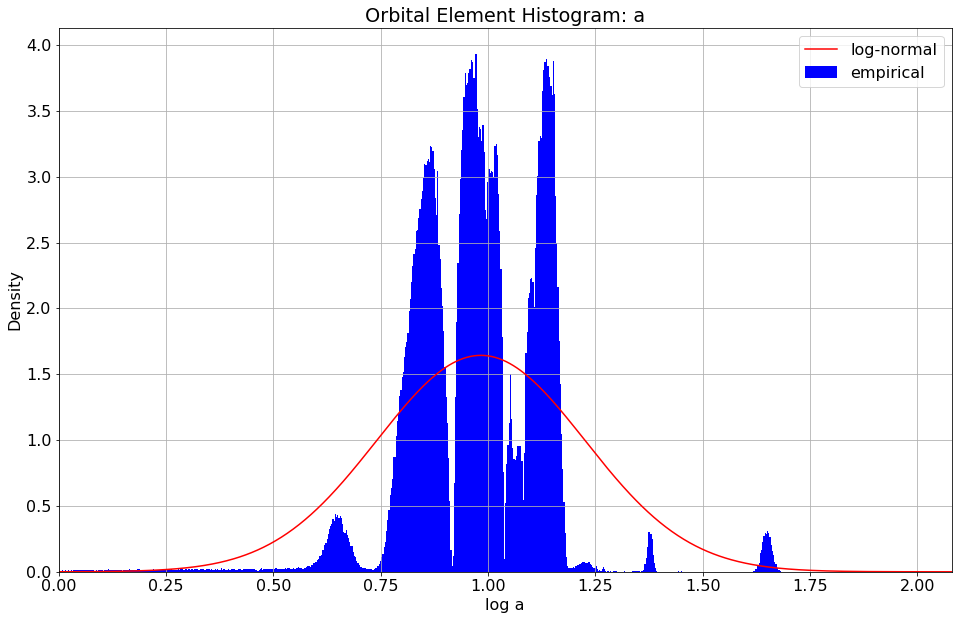
\includegraphics[width=1.0\textwidth]{../figs/elts/elt_hist_a_pdf.png}
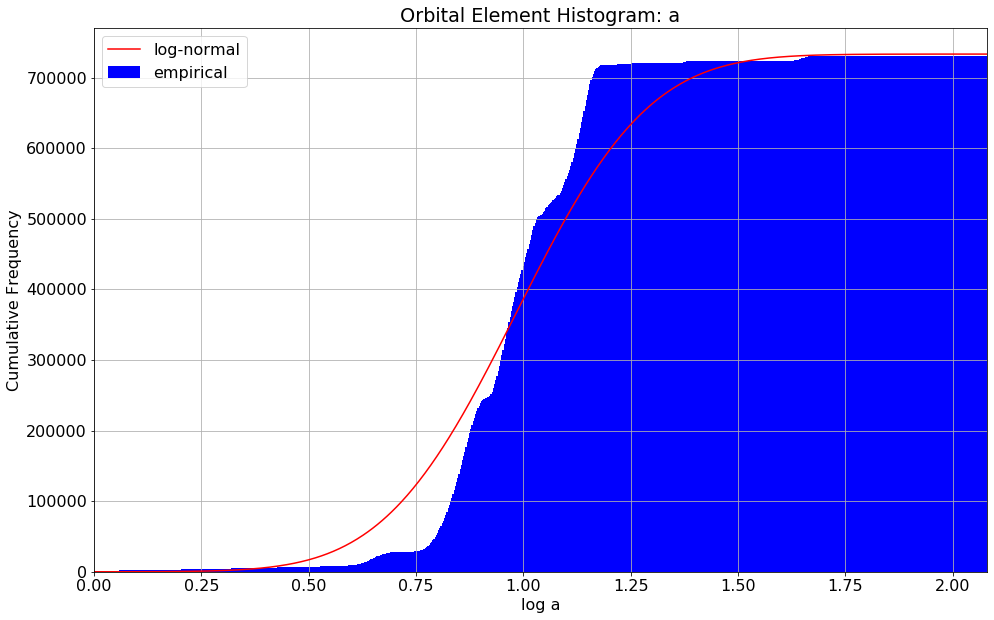
\includegraphics[width=1.0\textwidth]{../figs/elts/elt_hist_a_cdf.png}
\caption{PDF and CDF for $\log(a)$, log of the semi-major axis.\\
We can clearly see the famous Kirkwood gaps in the PDF. \\
The CDF shows that on a macroscopic scale, a log-normal model isn't bad.\\
$\log(a)$ is sampled empirically from the CDF.}
\end{center}
\end{figure}
\clearpage

\begin{figure}[hbt!]
\begin{center}
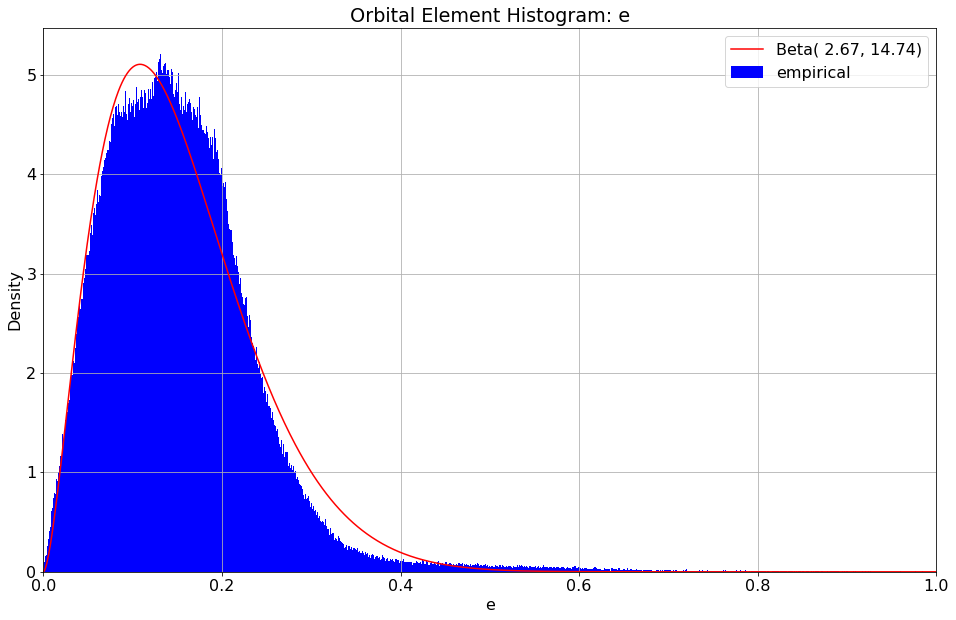
\includegraphics[width=1.0\textwidth]{../figs/elts/elt_hist_e.png}
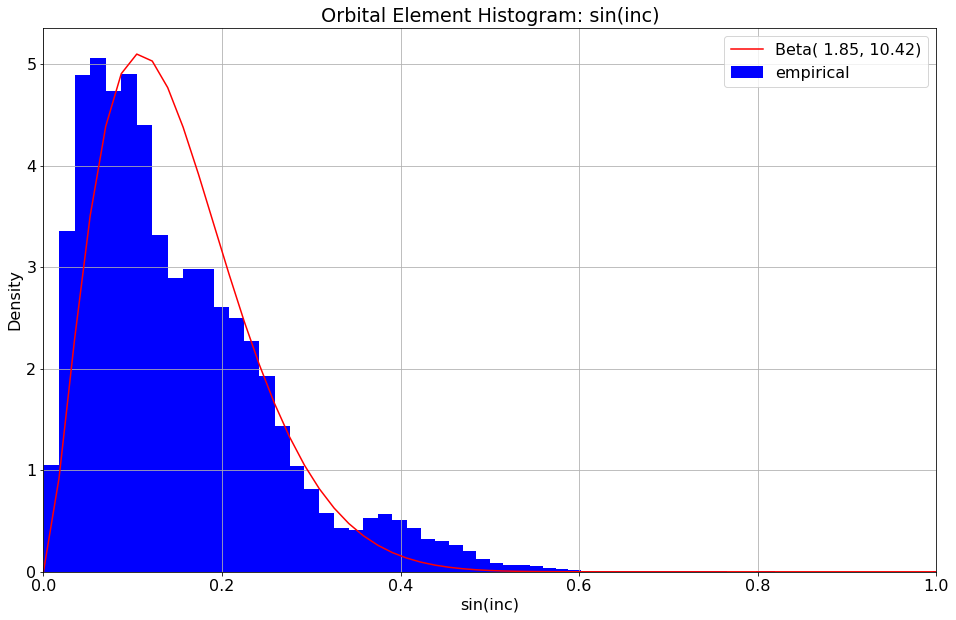
\includegraphics[width=1.0\textwidth]{../figs/elts/elt_hist_i.png}
\caption{PDF for eccentricity $e$ and $\sin(i)$ (sine of the inclination).\\
Both $e$ and $\sin(i)$ are bounded in $[0, 1]$ and can be decently approximated by a Beta distribution.\\
Boith $e$ and $i$ are sampled empirically from the CDF; Beta sampling could have also worked well.}
\end{center}
\end{figure}
\clearpage

\begin{figure}[hbt!]
\begin{center}
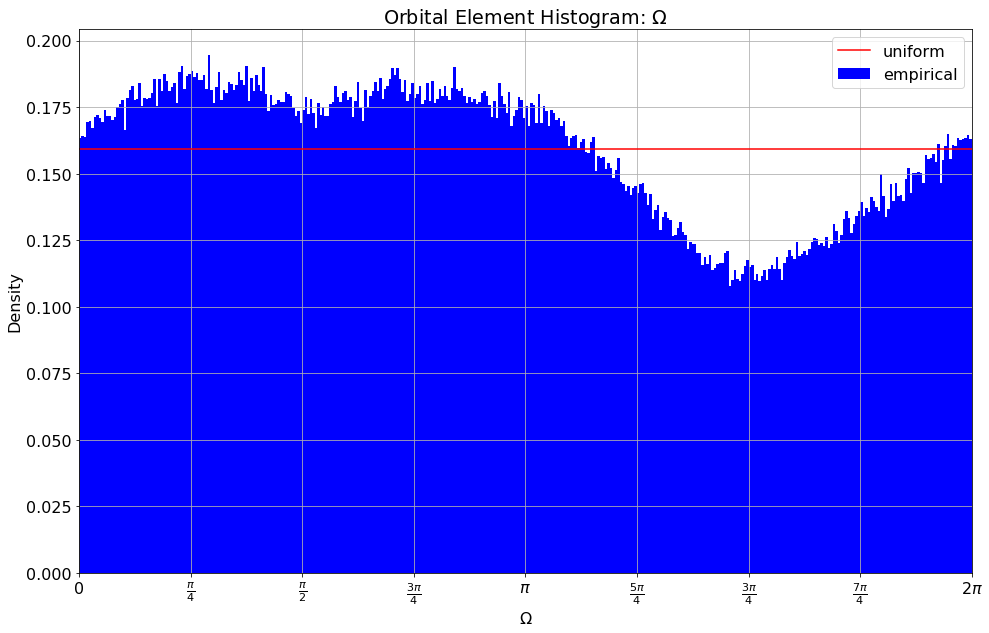
\includegraphics[width=1.0\textwidth]{../figs/elts/elt_hist_Omega_node.png}
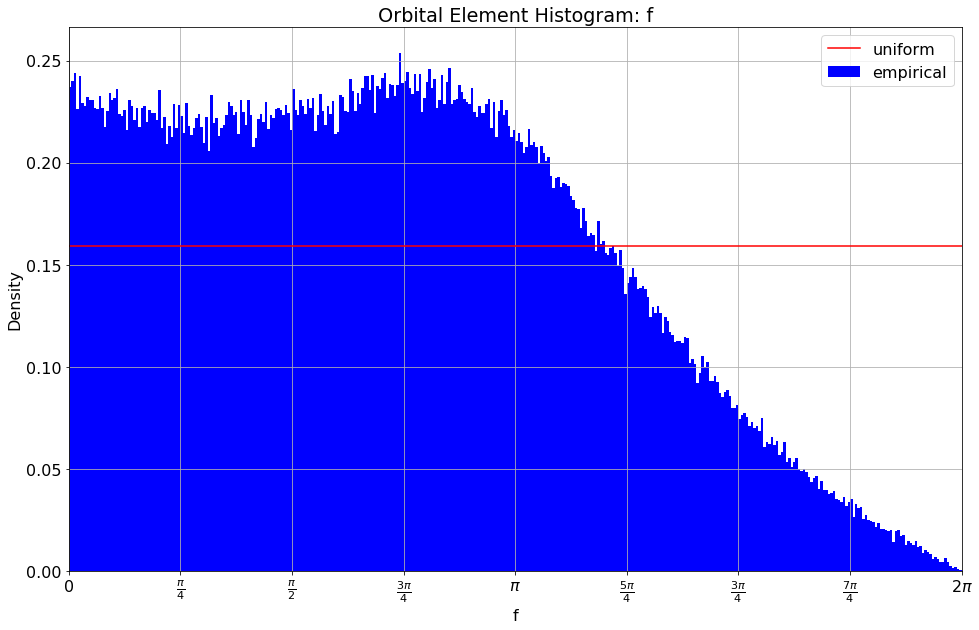
\includegraphics[width=1.0\textwidth]{../figs/elts/elt_hist_f.png}
\caption{PDF for longitude of ascending node $\Omega$ and true anomaly $f$.\\ 
The PDF for $\Omega$ is somewhat close to uniform, but with a noticeable departure.\\
The PDF for $f$ has an odd shape that I would have been hard pressed to predict ahead of time.\\
$\Omega$ is sampled empirically from the CDF; $f$ is computed by sampling $M$ uniformly.}
\end{center}
\end{figure}
\clearpage

\begin{figure}[hbt!]
\begin{center}
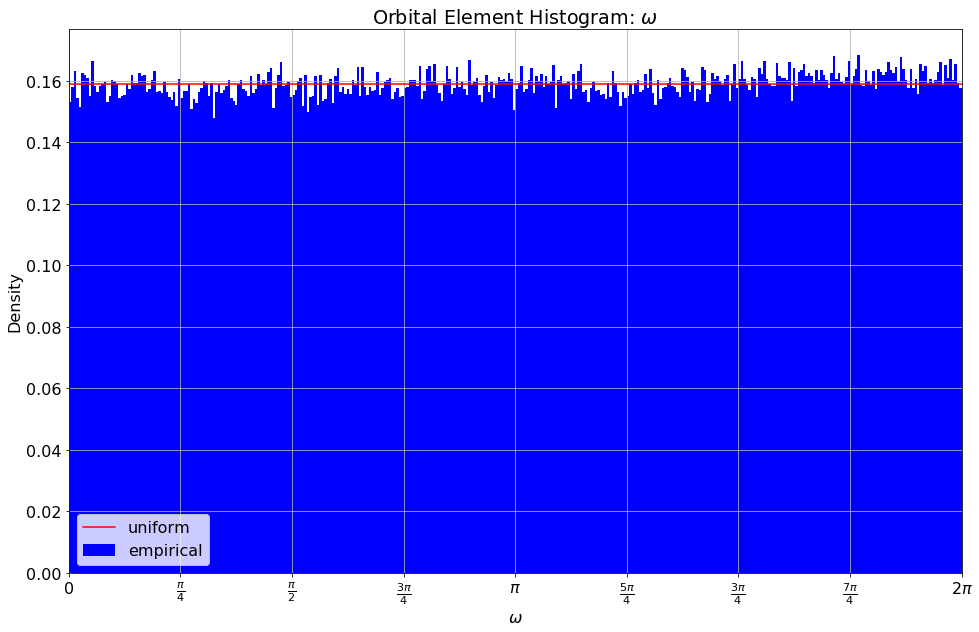
\includegraphics[width=1.0\textwidth]{../figs/elts/elt_hist_omega_peri.png}
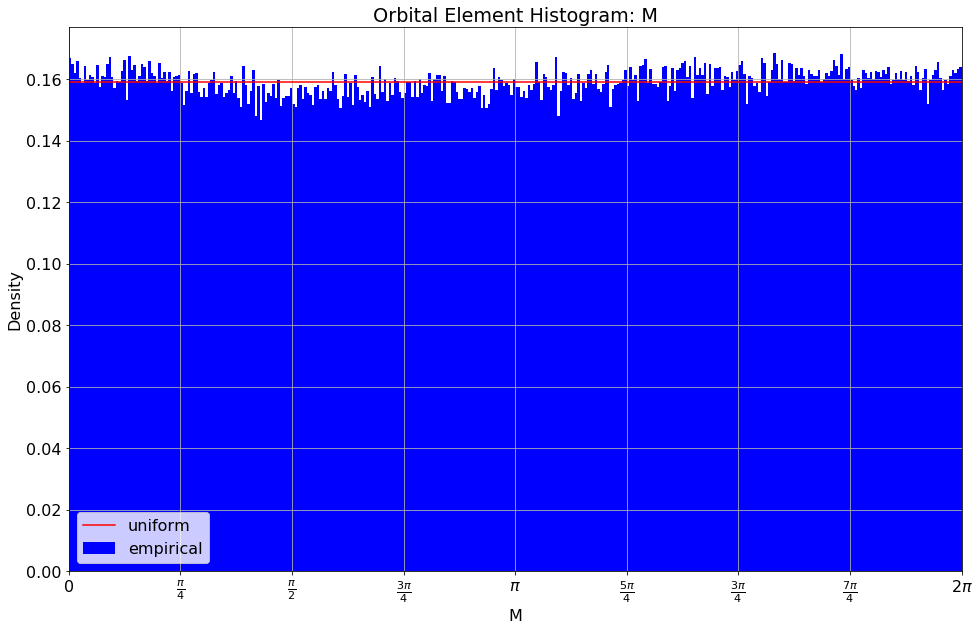
\includegraphics[width=1.0\textwidth]{../figs/elts/elt_hist_M.png}
\caption{PDF for argument of perihelion $\omega$ and mean anomaly $M$.\\ 
As promised, these are empirically very close the uniform distribution we would expect.\\
Both of these elements are sampled uniformly at random..}
\end{center}
\end{figure}
\clearpage

If a continuous rather than discrete sampling strategy were desired, $e$ and $\sin(inc)$ could be well approximated by 
a fitted Beta distribution as shown in the preceding charts.
Drawing $\log(a)$ from a distribution could be a bit messy.  
To my eye the best solution there would be a mixture of normals with perhaps $6$ to $10$ components.
I see little argument in favor of drawing $a$ or $\omega$ other than empirically.
Random elements are generated in the module \tty{candidate\_elements.py} with the function \tty{random\_elts}.
A random seed is used for reproducible results.

\section{Assembling ZTF Detections Near Candidate Elements}
\label{section_ztf_elements}
Once we've generated a set of candidate orbital elements, 
the next step in the computation is to find all the ZTF detections that lie within a given threshold of the elements.
We've already introduced the important ideas that go into this computation in earlier sections.
The only difference is that instead of calculating the direction of a known asteroid whose orbit was integrated and saved to disk, 
we integrate the orbit of the desired elements on the fly.
Then we proceed to calculate the predicted direction from the Palomar observatory and filter down to only those within the threshold
(I used 2.0 degrees in the large scale search.)

The module \tty{ztf\_element} includes a function \tty{load\_ztf\_batch} that takes as arguments dataframes \tty{elts} and \tty{ztf}
of candidate orbital elements and ZTF observations to cross reference against.
It also takes a threshold in degrees.
It returns a data frame of ZTF elements that is keyed by \tty{(element\_id, ztf\_id)}
where \tty{element\_id} is an identifier for one candidate element (intended to be unique across different batches)
and \tty{ztf\_id} is the identifier assigned to each ZTF detection.

The work of integrating the candidate elements on a daily schedule is carried out by \tty{calc\_ast\_data} In module \tty{asteroid\_dataframe}.
The work of splining the daily integrated asteroid positions and velocities at the distinct observation times is done in \tty{make\_ztf\_near\_elt}.
Because this computation is fairly expensive (it takes about 25 seconds to integrate a batch of 64 candidate elements),
a hash of the inputs is taken and the results are saved to disk using the hashed ID.
If a subsequent call for the ZTF elements is made with the same elements, it is loaded from the cache on disk.

Those readers who would like an interactive demonstration can find one in the Jupyter notebook \tty{06\_ztf\_element.ipynb}.
Here is a preview of the output dataframe \tty{ztf\_elt}:
\begin{figure}[hbt!]
\begin{center}
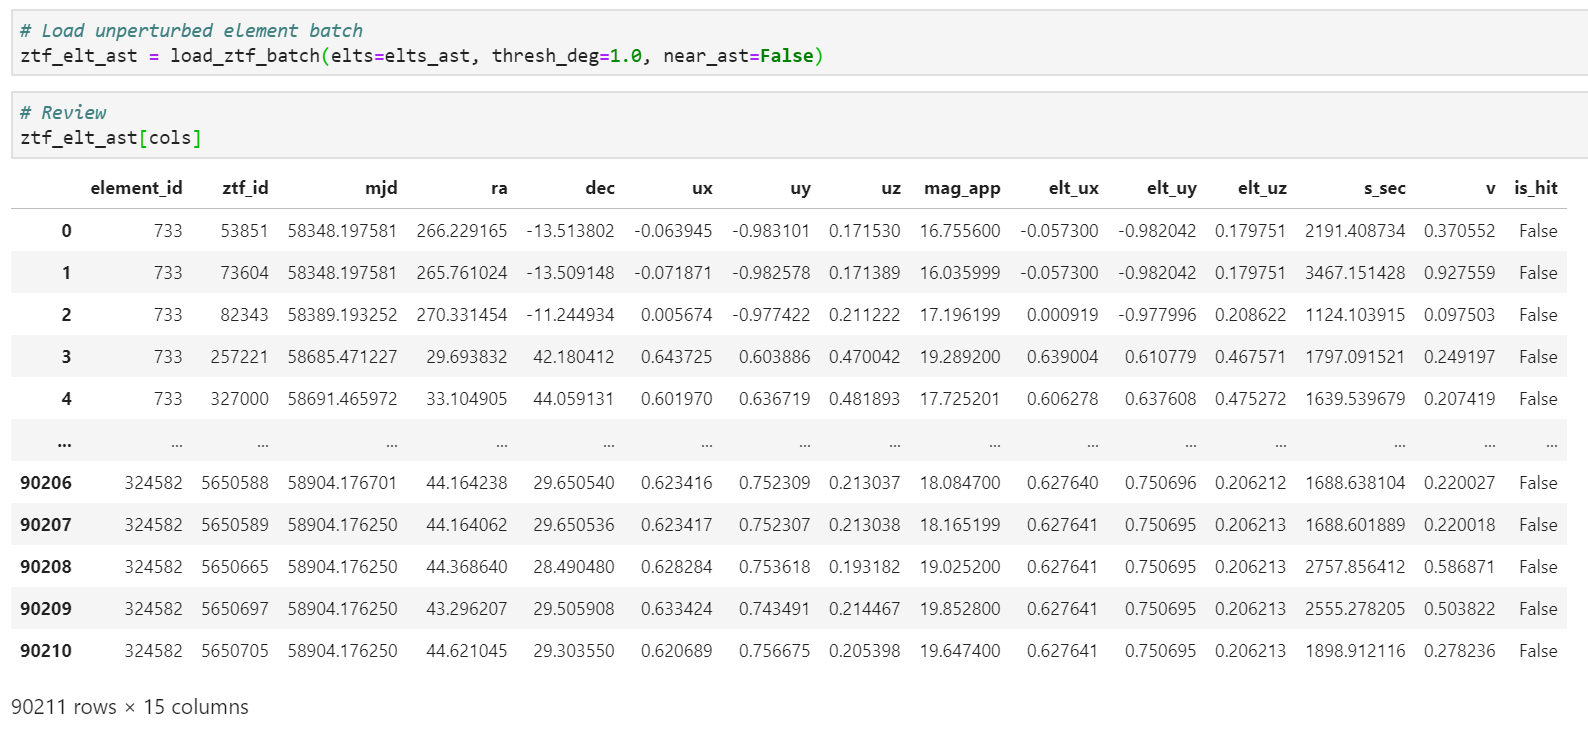
\includegraphics[width=1.0\textwidth]{../figs/elts/ztf_elt_dataframe.png}
\caption{ZTF detections within a 1.0 degree threshold of a batch of 64 orbital elements.}
\end{center}
\end{figure}

In Chapter 3, we showed that the quantity $v = (s/\tau)^2$ is would be distributed $\sim \Unif[0,1]$
if predicted distributions were distributed uniformly at random.
The function \tty{plot\_v} in module \tty{element\_eda} generates such a plot.
I generated a list of the 64 asteroids that have the most hits in the ZTF dataset (ranging from 148 to 194).
Then I generated ZTF dataframes for three collections of orbital elements: 
\begin{itemize}
\item unperturbed orbital elements belonging to these 64 asteroids
\item perturbed orbital elements of these 64 asteroids
\item random orbital elements
\end{itemize}
As a test of the theory and to build intuition, I plot the distribution of $v$ against the original threshold of 1.0 degree.
The results are exactly as predicted.
The random distribution is approximately uniform as expected.
The unperturbed distribution is a mixture of uniform and a spike in the first bucket.
The perturbed distribution is in between, with the hits leaking out over the first few buckets out to $v \approx 0.07$ (about 250 arc seconds).
\begin{figure}[hbt!]
\begin{center}
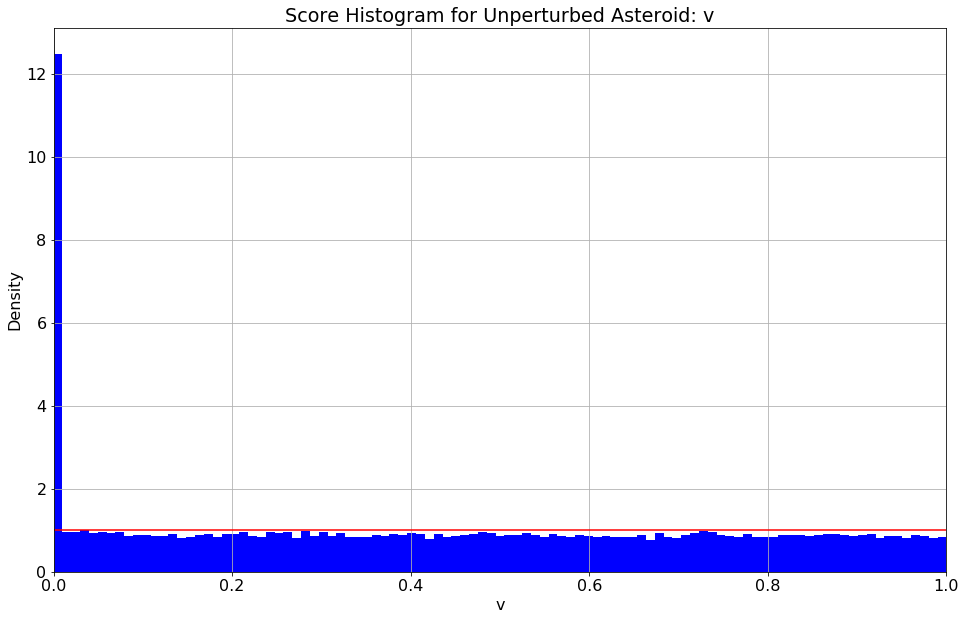
\includegraphics[width=0.70\textwidth]{../figs/elts/v_hist_unperturbed.png}
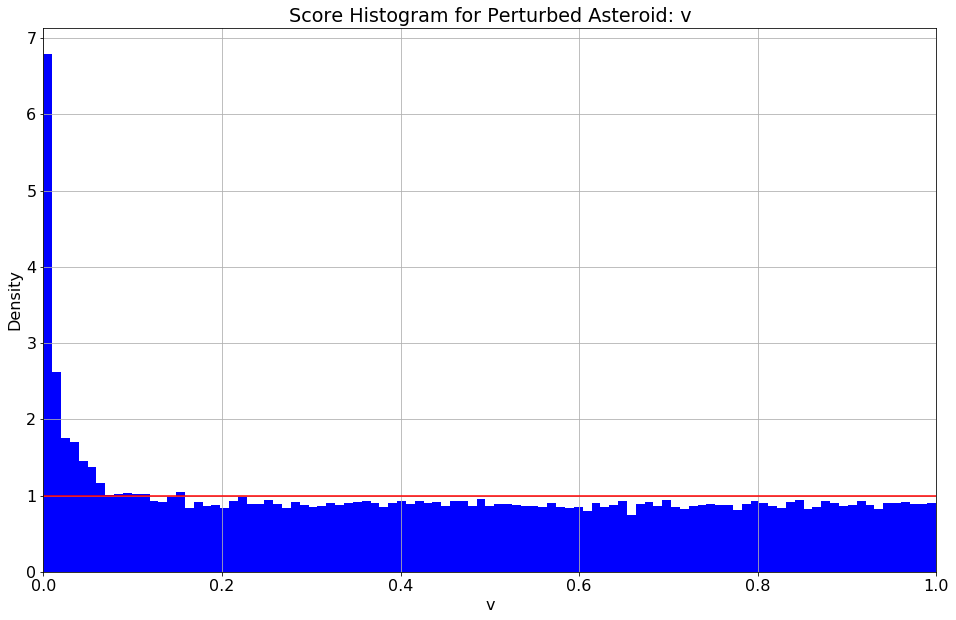
\includegraphics[width=0.70\textwidth]{../figs/elts/v_hist_perturbed.png}
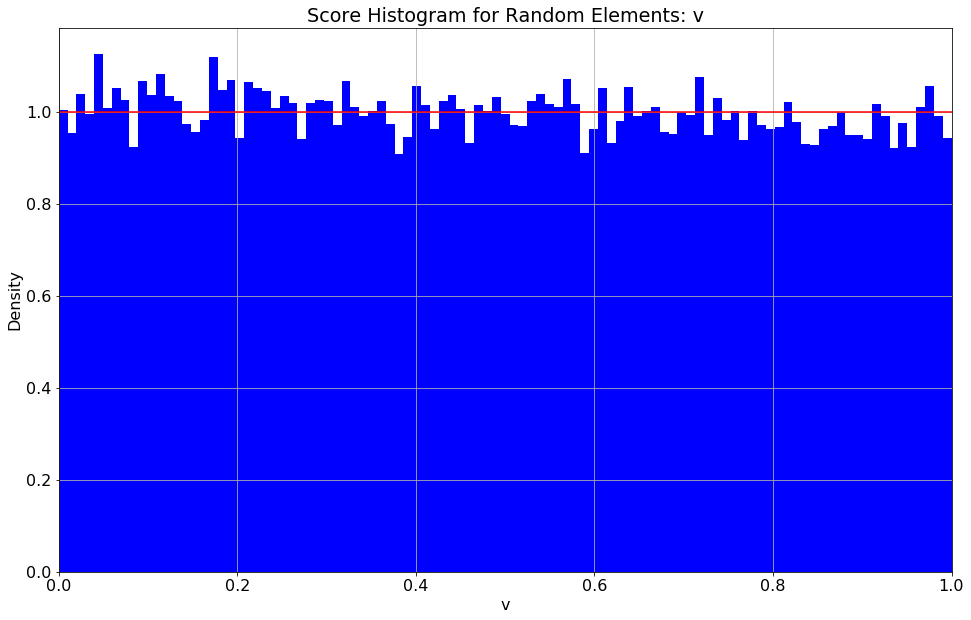
\includegraphics[width=0.70\textwidth]{../figs/elts/v_hist_random.png}
\caption{Histogram of $v = (s/\tau)^2$ for three sets of candidate orbital elements.}
\end{center}
\end{figure}
\clearpage

\section{Filtering the Best Random Elements}
\label{section_best_random_elements}
One idea is to perform a preliminary screening of the candidate orbital elements 
before investing a large amount of computational resources into running an aseteroid search on them.
In the next section we will show how to generate the ZTF detections within a threshold $\tau$ of the candidate elements.
We've already seen that the random variable $V = (S/ \tau)^2$ is distributed $V \sim \Unif(0, 1)$.
One idea is to assess candidate elements by taking the sample mean of $\log(v)$;
we want to explore elements that have a disproportionate share of hits where $v$ is small.
Here is a quick demonstration that for $V \sim \Unif(0,1)$, $\log(V)$ has expectation $-1$ and variance $1$.
\begin{align*}
\E[ V ] &= \int_{v=0}^{\infty} \log (v) dv = \left. v \log v - v \right]_{0}^{1} = (1 \cdot \log 1 - 1) - (0 - 0) = -1 \\
\Var[V ] &= \E[V^2] - \E[V]^2 = \int_{v=0}^{1} \log(v)^2 dv - (-1)^2 \\
&= \left. v \cdot (\log v)^2 - 2 \log v + 2) \right]_{0}^{1} = 2 -1 = 1
\end{align*}
If a set of candidate elements has $n$ detections within threshold $\tau$ with relative squared distances of $v_1, \ldots v_n$,
their sample mean $\bar{v}$ will have expectation $-1$ and variance $n$, so I contruct a t-score for candidate elements
$$T = \frac{-(\bar{v} + 1)}{n}$$
This score would be distributed $T \sim \mathrm{N}(0, 1)$ (standard normal) if the guessed positions were uniformly random.
It provides a computationally efficient way to screen candidate orbital elements.

This screening is performed in the module \tty{random\_elements}.
The function \\
\tty{calc\_best\_random\_elts} generates a large batch of random elements (the default size is 1024).
It then builds the ZTF observations close to them and extract the t-score as described above.
The input batch size is used to select that many of the candidates that have the best score.
The whole process of building the ZTF data frames, searching for the best elements,
and saving the best elements and assembled ZTF data frames to disk is carried out by a Python program that can be run from the command line as
\begin{lstlisting}[style=CodeSnippet]
(kepler) $ python random_elements.py -seed0 0 -seed1 1024 -stride 4 
> -batch_size_init 1024 -batch_size 64 -known_ast
\end{lstlisting}
The example call above runs the program on 256 batches of random elements, with random seeds $[0, 4, \ldots, 1020]$.
The stride argument is to facilitate parallel processing.
The two batch size arguments request that $1024$ initial elements be winnowed down to $64$ with the highst t-scores.
The flag \tty{-known\_ast} at the end asks that only the subset of ZTF detections within 2.0 arc seconds of a known asteroid be used 
to generate the ZTF dataframe and score the initial elements.
I call this searching against known asteroids.
If \tty{known\_ast} is not passed, the behavior is the opposite; only the ZTF detections at least 2.0 arc seconds (i.e. ones that don't closely match) are considered.
I ran this program to generate 4096 candidate elements for each of the known and unknown asteroids.
Altogether it took quite a while to run, over one day of total computer time.
The vast bulk of that time is spent building the ZTF dataframe of detections near the elements.

\section{Formulating the Log Likelihood Objective Function}
\label{section_log_likelihood}
The actual asteroid search is an optimization performed in TensorFlow using gradient descent.
Perhaps the most important choice is that of the objective function.
Qualitatively we know that we want an objective function that will be large when we are very close 
(within a handful of arc seconds) to some of the detections.
We don't have a preference about the distance to the other detections.
While it might seem tempting to write down an objective that rewards being close to everything, that's not at all what we want.
Such an objective function would encourage us to find some kind of ``average orbital element'' for all the asteroid detections  in this collection.
But we want to find the elements of just one real asteroid.

A principled way to formulate an objective function is with probability.
As a reminder, $S$ is the Cartesian distance between $\upred$ and $\uobs$,
and $\tau$ is the threshold Cartesian distance so only observations with $S < \tau$ are considered.
$V = S / \tau$ is in the interval $[0, 1]$.
Introduce the following probability mixture model for the random variable $V$.
Some unknown fraction $h$ (for hits) of the observations are associated with one real asteroid, whose elements we are converging on.
Conditional on an observation being in this category (a hit), the distribution of $V$ is exponential with paramter $\lambda$.
Conditional on an observation being a miss, $V$ is distributed uniformly on $[0,1]$.
In the formalism of conditional probability,
\begin{align*}
V | Hit &\sim \Expo(\lambda) \\
V | Miss &\sim \Unif(0,1)
\end{align*}
We can relate the parameter $\lambda$ to a resolution parameter $R$ by observing that $v=(s/\tau)^2$ and
$$f(v) \propto e^{-\lambda v} = e^{-\lambda s^2 / \tau^2}$$
This looks just like a normal distribution in the Cartesian distance $s$, a plausible and intuitive result!
Let us identify the standard deviation parameter $\sigma$ of this normal distribution with the resolution $R$,
i.e. think of the PDF $f(s)$ as being normal with PDF $f(x) \propto e^{-s^2 / 2 R^2}$.\\
Equating the exponent in both expressions, we get the relationship
$$ \lambda = \frac{\tau^2}{2R^2}$$

It is convenient to use $\lambda$ for calculations, both mathematical and in the code.
For understanding what is going on, I find it more intuitive to use the resolution, since it's on the same scale as the threshold $\tau$.
The PDF of an exponential distribution is given by \cite{BH}
$$ f(v; \lambda) =\lambda e^{-\lambda v}$$
In this case, we need to modify this PDF slightly to account for the fact that $v \in [0,1]$ 
while the support the exponential distribution is $[0, \infty)$.
What we want instead is the truncated exponential distribution, which is normalized to have probability $1$ on the interval $[0,1]$, namely
$$ f(v| \mathrm{Hit}, \lambda) = \frac{\lambda v}{1 - e^{-\lambda}}$$
Of course, the PDF of the uniform distribution is just $1$, so
$$ f(v | \mathrm{Miss}) = 1$$
Now we can write the PDF of the mixture model using the Law of Total Probability:
\begin{align*}
f(v| h, \lambda) &= f(v|\mathrm{Hit}, \lambda) \cdot P(\mathrm{Hit}) + f(v|\mathrm{Miss}) \cdot P(\mathrm{Miss}) \\
&= h \cdot \frac{\lambda v}{1 - e^{-\lambda}} + 1 - h
\end{align*}

The optimization objective function will be the log likelihood of the PDF:
$$ \mathcal{L}(\vvec, h, \lambda) = \sum_{j=1}^{n} \log \left( h \cdot \frac{\lambda v_j}{1 - e^{-\lambda}} + 1 - h \right)$$
Please note that I've omitted the parameter $\tau$ from these expressions to lighten the notation.
During the training of the model, the $\tau$ parameter is also updated.
The three mixture parameters that are manipulated during training are 
\begin{itemize}
\item \tty{num\_hits}: the number of hits for this candidate element
\item $R$: the resolution of this candidate element as a Cartesian distance
\item $\tau$: the threshold of this candidate element as a Cartesian distance
\end{itemize}
The hit rate $h$ is computed from \tty{num\_hits} by dividing by the number of rows that are within the threshold distance.
The dimensionless error term $v$ is computed by taking $v = (s/\tau)^2$.
The exponential decay parameter $\lambda$ is calculated as $\lambda = \tau^2 / 2R^2$.

In general, a likelihood function is only defined up to a multiplicative factor and a log likelihood up to an additive constant.
In a theoretical analysis of maximum likelihood, the constant is typically irrelevant because one is differentiating the likelihood function anyway.
In this problem, I want to set the constant term so that a log likelihood of zero equates to having no information,
i.e. an uniformative baseline.
This is particularly easy to do here: if we set $h=0$, the terms involving the truncated exponential distribution all drop out 
and the log likelihood becomes a sum of $\log(h) = 0$.
In general, we can zero out the log likelihood function by evaluating it at a set of uninformative baseline values, 
and subtracting this quantity $\mathcal{L}_0$ from the current optimized $\mathcal{L}$.

This likelihood function applies to only one of the candidate orbital elements.
In the actual optimization of a batch of 64 elements, we need a single scalar valued objective function.
Because all of the elements in a batch are being optimized independently and have no interaction with each other, we can simply take their sum.
There is an important refinement to this idea though that I will discuss in the next section.

\todo{Add magnitude}

\section{Performing the Asteroid Search}
\label{section_asteroid_search}

\section{Recovering the Elements of Known Asteroids}
\label{section_results_known_ast}

\section{Presenting [N] Previously Unknown Asteroids}
\label{section_results_unknown_ast}

\section{Conclusion}
\label{search_conclusion}

\section{Future Work}
\label{section_future_work}

